% !TEX encoding = UTF-8 Unicode
% !TEX TS-program = pdflatex

% toptesti document class
\documentclass[%
    a4paper, % not needed, by default it is a4paper, or also b5paper can be used
    corpo=12pt, % dimension of basic font
    % oneside is generally the way to go
    oneside, % two side optimizes for two-face printing, having chapters open on the right (aka odd numbers), if you don't want blank pages put oneside here
    stile=standard,
    %evenboxes, % not needed, to put supervisors and candidate at the same level
    tipotesi=magistrale,
    numerazioneromana, % roman numbering for appendixes and preambles, up to Table of Contents
    openright, % to force opening on the right for double-sided printing
    cucitura=7mm, % for printing, 7mm should be enough
    %dvipsnames, % for compatibility with xcolor, it does not work
]{toptesi}


%%%%%%%%%%%%%%%%%%%%%%%%%%%%%%%%%%%%%%%%%%%%%%%%%%%%
\usepackage[english]{babel}
\usepackage[utf8]{inputenc}
\usepackage[T1]{fontenc}
\usepackage{lmodern}

\usepackage{hyperref} % must be loaded before glossaries-extra

% bibliography
\usepackage[hyperref=true,backref=true,backend=biber,maxbibnames=9,maxcitenames=2,style=numeric,citestyle=numeric,sorting=none]{biblatex} % hyperref uses links, backref goes back to citations, uses biber as backend, with 9 names at most in bibliography and 2 in citations, citing using numbers, and sorting in citation order
% sorting can be also ydnt for year descending, name, title or ynt for ascending year

\usepackage{adjustbox} % to resize boxes by keeping the same aspect ratio
\usepackage{algorithm} % algorithm environment
\usepackage{algpseudocode} % improved pseudo-code
\usepackage{amsfonts}               %  AMS mathematical fonts
\usepackage{amsmath}
\usepackage{amssymb}                %  AMS mathematical symbols
\usepackage{bm}                     %  black/bold mathematical symbols
\usepackage{booktabs}               %  better tables
\usepackage[labelfont=bf]{caption} % font=footnotesize % to have reduced caption font size
\usepackage{csquotes}
\usepackage{enumitem} %left align the bulleted points
\usepackage{geometry}
%\usepackage{glossaries} % to use acronyms and glossary, it has also glossaries-extra as extension, but commands are different
\usepackage[%
    toc, % puts the link in the ToC
    %record, % to use bib2gls
    abbreviations, % to load abbreviations / acronyms
    nonumberlist, % to avoid printing the numbers of the references in the acronyms page
]{glossaries-extra}
\usepackage{graphicx}               %  post-script images
%\usepackage{iwona} % extra fonts, substitute standard ones
\usepackage{listings} % to insert formatted code
\usepackage{lipsum} % for lorem ipsum text, not needed in the real work
\usepackage{makecell} % to change dimensions of cells, for math cases
\usepackage{mathtools} % for additional commands
\usepackage{mfirstuc} % to have capitalization capabilities
\usepackage[final]{microtype}      % microtypography, final lets latex use it also in bibliography
\usepackage{multirow} % to allow for cells covering more than 1 row in tables
\usepackage{nicefrac}       % compact symbols for 1/2, etc.
%\usepackage[lofdepth,lotdepth]{subfig}
\usepackage{ragged2e} % for justifying text
\usepackage{siunitx} % support for SI units of measurement and number typesetting
\usepackage{subfig}
\usepackage{svg} % for svg support, works only if inkscape is installed, default for Overleaf v2
%\usepackage{subfigure}              %  subfigure compatibility, can be removed if subfig
\usepackage{tabularx} % equal-width columns in tables
\usepackage{textcomp} % extra fonts and symbols
\usepackage{url}            % simple URL typesetting
\usepackage{verbatim} % for extended verbatim support
\usepackage{xcolor} % to define colors and use standard CSS names add dvipsnames as option, but it clashes with xcolor loaded in toptesi, pay attention that if it goes in conflict with tikz/beamer, simply use \documentclass[usenames,dvipsnames]{beamer}, along with other custom options when defining the document class


\usepackage{graphicx}
\usepackage{adjustbox}

\usepackage{tikz-timing}
\usetikztiminglibrary[rising arrows]{clockarrows}
\usetikzlibrary{automata, positioning}

\usepackage{breqn}



% \setlength\textwidth{7in}
% \setlength\textheight{10in}
% \setlength\oddsidemargin{(\paperwidth-\textwidth)/2 - 1in}
% \setlength\topmargin{(\paperheight-\textheight
% -\headheight-\headsep-\footskip)/2 - 1in}

% this configuration is close to TopTesi in width
% \newgeometry{a4paper,top=3cm,bottom=3cm,left=3cm,right=3cm,%
% heightrounded}
% margins as for libreoffice writer
\newgeometry{top=2cm,bottom=2cm,left=2cm,right=2cm,%
heightrounded}



% how to change Contents to Table of Contents
\addto\captionsenglish{% Replace "english" with the language you use
  \renewcommand{\contentsname}%
    {Table of Contents}%
}

% to change the name of Abbreviations to Acronyms
% not needed if use use entry types and define those
% \renewcommand{\abbreviationsname}{Acronyms}

% to allow line comments in algorithms
\algnewcommand{\LineComment}[1]{\State \(\triangleright\) #1}

% to declare abs and norm
\DeclarePairedDelimiter\abs{\lvert}{\rvert}%
\DeclarePairedDelimiter\norm{\lVert}{\rVert}%

% Swap the definition of \abs* and \norm*, so that \abs
% and \norm resizes the size of the brackets, and the 
% starred version does not.
\makeatletter
\let\oldabs\abs
\def\abs{\@ifstar{\oldabs}{\oldabs*}}
%
\let\oldnorm\norm
\def\norm{\@ifstar{\oldnorm}{\oldnorm*}}
\makeatother


% change this configuration with your info
% if you need fewer or more supervisors you have to change \relatore command by adding or removing lines in the table in toptesi_config
\newcommand{\thesistitle}{Study and development of fault tolerant operating systems on FPGA for aerospace applications}
\newcommand{\thesisuniversitylogo}{images/logo/polytechnic-university-of-turin-logo_clipped} % choose your logo
\newcommand{\thesiscandidatename}{Salvatore Gabriele}
\newcommand{\thesiscandidatesurname}{La Greca}
\newcommand{\thesissupervisoronetitle}{Prof.}
\newcommand{\thesissupervisoronename}{Luca}
\newcommand{\thesissupervisoronesurname}{Sterpone}
\newcommand{\thesissupervisortwotitle}{Ing.}
\newcommand{\thesissupervisortwoname}{Daniele}
\newcommand{\thesissupervisortwosurname}{Rizzieri}
\newcommand{\thesissupervisorthreetitle}{Ph.D}
\newcommand{\thesissupervisorthreename}{Sarah}
\newcommand{\thesissupervisorthreesurname}{Azimi}
\newcommand{\thesisdate}{July 2022}
\newcommand{\thesiscourse}{Computer Engineering}
\newcommand{\thesisuniversity}{Politecnico di Torino}
\newcommand{\thesislevel}{Master} % master or bachelor
\newcommand{\thesiscandidatetext}{Candidate}
\newcommand{\thesissupervisortext}{Supervisors}


% fontsize is {size}{spacing}\family
\newcommand {\institutionfont}{\fontsize {22}{30}\scshape}
\newcommand {\divisionfont}{\fontsize {16}{20}\rmfamily}
\newcommand {\pretitlefont}{\fontsize {16}{16}\rmfamily}
\newcommand {\customtitlefont}{\fontsize {21}{28}\scshape}% {iwona}{bx}{n}}
\newcommand {\fixednamesfont}{\fontsize {14}{20}\mdseries}
\newcommand {\namesfont}{\fontsize {14}{20}\bfseries}
\newcommand {\footfont}{\fontsize {15}{18}\rmfamily}


\usepackage{xcolor, bytefield}

% facilitates the creation of memory maps. Start address at the bottom,
% end address at the top.
% syntax:
% \memsection{end address}{start address}{height in lines}{text in box}
\newcommand{\memsection}[4]{%
% define the height of the memsection
\bytefieldsetup{bitheight=#3\baselineskip}%
\bitbox[]{10}{%
\texttt{#1}% print end address
\\
% do some spacing
\vspace{#3\baselineskip}
\vspace{-2\baselineskip}
\vspace{-#3pt}
\texttt{#2}% print start address
}%
\bitbox{16}{#4}% print box with caption
}

\definecolor{codegreen}{rgb}{0,0.6,0}
\definecolor{codegray}{rgb}{0.5,0.5,0.5}
\definecolor{codepurple}{rgb}{0.58,0,0.82}
\definecolor{codered}{rgb}{0.8,0,0}
\definecolor{backcolour}{rgb}{0.95,0.95,0.92}
\definecolor{NavyBlue}{rgb}{0,0,0.5}
\definecolor{orange}{rgb}{1,0.5,0}

\lstdefinestyle{preformatted}{
    backgroundcolor=\color{backcolour},   
    commentstyle=\color{codegreen},
    keywordstyle=\color{magenta},
    numberstyle=\tiny\color{codegray},
    stringstyle=\color{codepurple},
    basicstyle=\ttfamily\footnotesize,
    breakatwhitespace=false,         
    breaklines=true,                 
    captionpos=b,                    
    keepspaces=true,                 
    numbers=left,                    
    numbersep=5pt,                  
    showspaces=false,                
    showstringspaces=false,
    showtabs=false,                  
    tabsize=2
}

\lstdefinestyle{tcl}{
    backgroundcolor=\color{backcolour},   
    commentstyle=\color{codegreen},
    % keywordstyle=\color{red},
    numberstyle=\tiny\color{codegray},
    stringstyle=\color{codepurple},
    basicstyle=\ttfamily\footnotesize,
    language=tcl,
    breakatwhitespace=false,         
    breaklines=true,                 
    captionpos=b,                    
    keepspaces=true,                 
    numbers=left,                    
    numbersep=5pt,                  
    showspaces=false,                
    showstringspaces=false,
    showtabs=false,                  
    tabsize=2,
    morekeywords={*, create_pblock, get_pblocks, add_cells_to_pblock, get_cells, resize_pblock, set_property, open_run, write_bitstream, get_designs},
    literate=*{\{}{{\textcolor{red}{\{}}}{1}
        {\}}{{\textcolor{red}{\}}}}{1}
        {[}{{\textcolor{red}{[}}}{1}
        {]}{{\textcolor{red}{]}}}{1}
        {(}{{\textcolor{red}{(}}}{1}
        {)}{{\textcolor{red}{)}}}{1}%
}


\addbibresource{bibliography.bib}

% to load the glossaries, not needed if using bib2gls
% for glossary entry
% @entry{bird,
%     name={bird},
%     description = {feathered animal},
%     see={[see also]{duck,goose}}
% }

% if this bib file does not work, try using \input{file.tex}
% where all the \newabbreviation commands have been inserted
% containing all the definitions

% Gls to capitalize first letter
% GLS for full uppercase
% for abbreviations also
% glsxtrshort for abbreviation
% similar for long, full, and capital configurations, add pl at the end for plurals
% glsentryshort, long, plural (referred to shorts) must be used when in section titles
% glslink to allow the link but use a different text (as for href)


% if you want to use also description for the abbreviations/acronyms, you should use bib2gls and define all the entries in a bib file, which is incompatible with Overleaf
\newacronym{SEU}{SEU}{Single Event Upset}
\newacronym{COTS}{COTS}{Commercial Off-The-Shelf}
\newacronym{FPGA}{FPA}{Field Programmable Gate Array}
\newacronym{ASIC}{ASIC}{Application Specific Integrated Circuit}
\newacronym{CLB}{CLB}{Configurable Logic Block}
\newacronym{LAB}{LAB}{Logic Array Block}
\newacronym{LUT}{LUT}{Look-up Table}
\newacronym{HDL}{HDL}{Hardware Description Language}
\newacronym{CPU}{CPU}{Central Processing Unit}
\newacronym{DSP}{DSP}{Digital Signal Processing}
\newacronym{CMOS}{CMOS}{Complementary Metal-Oxide Semiconductor}
\newacronym{TMR}{TMR}{Triple Module Redundancy}
\newacronym{SEE}{SEE}{Single Event Effect}
\newacronym{SOC}{SOC}{System On Chip}


\makeglossaries

\begin{document}

\title{\vspace*{-5mm}\textbf{\thesistitle}\\Summary} % vspace is needed to shift upwards the title
\date{\thesisdate}
\author{\textbf{Candidate}:\\\thesiscandidatename~\thesiscandidatesurname\\
\textbf{Supervisors}:\\\thesissupervisoronetitle~\thesissupervisoronename~\thesissupervisoronesurname\\
\thesissupervisortwotitle~\thesissupervisortwoname~\thesissupervisortwosurname\\
\thesissupervisorthreetitle~\thesissupervisorthreename~\thesissupervisorthreesurname}


\ateneo{\thesisuniversity} % university name
\logosede[5cm]{\thesisuniversitylogo} % logo, square brackets contain the height

\titolo{\thesistitle} % title
%\sottotitolo{Metodo dei satelliti medicei} % subtitle

% place/remove a slash \\ to put the name on the following line or after Master Degree Course
\corsodilaurea{\thesiscourse} % course name


%~251197 % id number is not needed

\candidato{\thesiscandidatename~\textsc{\thesiscandidatesurname}} % candidate

% using tabular we can have more than 1 supervisor under the same column
\relatore{\tabular{@{}l}%
    \xmakefirstuc{\thesissupervisoronetitle}~\thesissupervisoronename~\textsc{\thesissupervisoronesurname}\\[0.4ex]
    \xmakefirstuc{\thesissupervisortwotitle}~\thesissupervisortwoname~\textsc{\thesissupervisortwosurname}\\[0.4ex]
    \xmakefirstuc{\thesissupervisorthreetitle}~\thesissupervisorthreename~\textsc{\thesissupervisorthreesurname}
    \endtabular}
%\terzorelatore{Ciao}

% in this way we have Academic Year without stile=classica, so without lines
%\sedutadilaurea{\textsc{Academic~Year} 2019-2020}% per la laurea magistrale
% for PoliTo there is only month year
\sedutadilaurea{\thesisdate}% per la laurea magistrale
% PhD
%\esamedidottorato{Novembre 1610}
%\ciclodidottorato{XV}

% offset for binding, the smaller the better
%\setbindingcorrection{3mm}


\english% or \italian (default)

\iflanguage{english}{%
	%\retrofrontespizio{This work is subject to the Creative Commons Licence}

	\CorsoDiLaureaIn{\thesislevel's Degree Course in\space}

	\TesiDiLaurea{\thesislevel's Degree Thesis}

	\InName{in}
	\CandidateName{\xmakefirstuc{\thesiscandidatetext}}% or Candidates
	\AdvisorName{\xmakefirstuc{\thesissupervisortext}}% or Supervisor
	%\TutorName{Tutor}
	%\NomeTutoreAziendale{Internship Tutor}

	%\NomePrimoTomo{First volume}
	%\NomeSecondoTomo{Second Volume}
	%\NomeTerzoTomo{Third Volume}
	%\NomeQuartoTomo{Fourth Volume}
}{}


% front page
% frontespizio can be used for the first page print
% while the custom-made frontpage can be used as hard-cover
% use pdfjoin or pdfseparate to extract or put together the pages if needed
%\frontespizio* % without star the logo is on top
\newgeometry{top=4cm,left=3cm,right=3cm,bottom=4cm,heightrounded}
\begin{titlepage}
\centering
%
{\institutionfont \textbf{\MakeUppercase{\thesisuniversity}} \par}
%
\vspace{\stretch{2}} % changing this number and the others changes the proportion
%
{\divisionfont \textbf{\thesislevel's Degree in \thesiscourse} \par}
%
\vspace{\stretch{3}}
%
\includegraphics[width=50mm]{\thesisuniversitylogo}\\
%
\vspace{\stretch{4}}
%
{\divisionfont \textbf{\thesislevel's Degree Thesis} \par}
%
\vspace{\stretch{3}}
%
{\customtitlefont \textbf{\thesistitle} \par}
%
\vspace{\stretch{10}}
%
\makebox[\textwidth]{\null\hfill\def\arraystretch{2}% % to change the spacing change this number
\begin{minipage}[t]{.375\textwidth}\raggedright
    \begin{adjustbox}{width={\textwidth},totalheight={\textheight},keepaspectratio} % with adjustbox it adapts to the lengths of the names, remove it if you want the same font dimension
    \begin{tabular}[t]{@{}l@{}}
        \fixednamesfont \textbf{\thesissupervisortext} \\
        \namesfont \xmakefirstuc{\thesissupervisoronetitle}~\thesissupervisoronename~\MakeUppercase{\thesissupervisoronesurname}\\
        \namesfont \xmakefirstuc{\thesissupervisortwotitle}~\thesissupervisortwoname~\MakeUppercase{\thesissupervisortwosurname}\\
        \namesfont \xmakefirstuc{\thesissupervisorthreetitle}~\thesissupervisorthreename~\MakeUppercase{\thesissupervisorthreesurname}
    \end{tabular}
    \end{adjustbox}
\end{minipage}
%
\hfill
%
\begin{minipage}[t]{.375\textwidth}\raggedleft
\begin{adjustbox}{width={\textwidth},totalheight={\textheight},keepaspectratio} % with adjustbox it adapts to the lengths of the names, remove it if you want the same font dimension
\begin{tabular}[t]{@{}l@{}}
    \fixednamesfont \textbf{\thesiscandidatetext} \\
    \namesfont \thesiscandidatename~\MakeUppercase{\thesiscandidatesurname}
\end{tabular}
\end{adjustbox}
\end{minipage}\hfill\null}\\
%
\vspace{\stretch{5}}
%
{\footfont \textbf{\thesisdate} \par}
%
\end{titlepage}

\restoregeometry
 % custom frontpage
%\retrofrontespizio
% insert text for the back of the front page
% if you insert any remove the following \paginavuota
% either a blank page or a back is needed to have double-sided printing
% pay attention to leave the space for the page

%\paginavuota % clears a page

\frontmatter

% abstract if needed
% \begin{abstract}
%     % abstract, choose between abstract and summary
% \end{abstract}

% to create blank pages for openright in frontmatter
% use one of the following two methods
% 1) use the following three lines
%\phantom{0} % needed otherwise cleardoublepage does not clean the page because it sees it empty
%\cleardoublepage
%\thispagestyle{empty} % to have empty page, without numbers
% 2) or
\paginavuota % to manually create a blank page

\sommario
% only the text for the summary
In the last few years, the number of missions devoted to universe exploration has increased. Predictions show that the amount of missions in the current decade is expected to be almost three times the amount of missions in the previous one, without considering low-cost and low-weight missions, like the ones including CubeSats. Therefore, the total quantity of electronic devices and the job complexity assigned to them is increasing as well.\bigskip

Electronic devices must be tailored to work reliably, whatever the purpose of a spacecraft, from the smallest one to a complete rover exploring another planet. Particularly, this concept holds in a complex environment like space, where there are many disturbances such as diverse temperature variations or radiations. The latter is one of the most common causes of failure in spacecrafts and the greatest enemy of electronic components. Thus, a system needs to be as dependable as possible. The dependability of a system is mainly affected by aspects like reliability, availability and safety, especially for space applications.\bigskip

Nowadays, FPGAs are increasingly being used in aerospace applications due to their flexibility: this is a key aspect of the success of missions because of their high costs, high duration and high complexity. As an example, the Mars Perseverance Rover is almost based on FPGAs. As an example, in the rover's architecture, an FPGA can be found in the automatic entry unit. This unit is responsible for the automatic entry, descent and landing on Mars. Once the rover is landed, it would be useless and would become dead hardware. However, it is based on FPGA hardware so it has been reprogrammed by NASA engineers from Earth to handle computer vision tasks. \bigskip

Consequently, this thesis aims to study and develop some techniques to mitigate errors induced in soft-cores by “Single Event Upset” faults, which are very common, especially in FPGAs. This area of interest is particularly crucial because complex software, like operating systems, running on top of this hardware, that may be faulty, can create uncoverable and dangerous situations. \bigskip

Before going deep into the argument, the thesis starts by explaining what an FPGA is, its differences from ASICs and the reason why the space industry is moving towards this technology. Furthermore, Chapter \ref{th-sec:background} introduces some concepts about radiations on electronic devices, how are they classified and what effects they can cause on a system. In addition to that, Chapter \ref{th-sec:backgroundthesis} introduces, with a great level of detail, all the tools and techniques used. The main purpose behind this chapter is to give to the reader a deeper knowledge of the arguments treated in this thesis work and to be able to recreate the proposed solution in the future, in almost a straightforward way. \bigskip

After that, the reader should be capable of understanding all the concepts that are mentioned in the main chapter of this thesis. Indeed, Chapter \ref{th-sec:main} analyzes different solutions that have been taken into consideration. The advantages and disadvantages of each solution are also discussed. Without entering into many details, the proposed solution aims to detect faults caused by SEUs in the Xilinx Microblaze CPU by using a custom peripheral. The custom peripheral has been developed in order to be fault-tolerant itself thanks to a Triple Module Redundancy design.\bigskip

Finally, when a fault is detected, a partial reconfiguration of the FPGA is triggered. This action consists of a partial scrubbing of the configuration memory of the FGPA, in the area where the MicroBlaze physically is. This is achieved by the usage of a partial bitstream, to restore the original behavior. The partial reconfiguration allows for achieving a faster downtime, and consequently a higher availability of the system. This process is entirely managed by the DFX (Dynamic Function Exchange) Controller IP, offered by Xilinx. The DFX Controller loads the configuration file from the memory and sends it to the configuration port of the FPGA. \bigskip

Moreover, a custom workflow has been developed to allow partial reconfiguration of a MicroBlaze in an older version of Vivado. Additionally, a custom script has been developed based on this workflow, thus providing designers and developers an easy and most automatized way to convert an existing Xilinx design into a design that supports the partial reconfiguration of the Microblaze.\bigskip

To conclude, Chapter \ref{th-sec:exp} and Chapter \ref{th-sec:concl} are devoted to the analysis of the results coming from this work and the analysis of the possible implications, applications and future work that can be done addressing further research interests.

% $400\times$ is nicer than 400x


\phantom{0}
\cleardoublepage
\thispagestyle{empty}

\ringraziamenti % acknowledgements
% acknowledgements

This thesis work would not be possible without the support of many people. I would like to thank my supervisors for their support and help in the development of this thesis.\bigskip

Thanks to my partner, Heidi G., for constantly listening to me rant and talk about strange things over and over, and for the sacrifices you have made and shared with me in order to help me pursue this Master's Degree. I also want to express my deep appreciation for Carol who taught me the importance of wit, sound sleep, and playfulness and for her cuddly, fidelity and love.\bigskip

Thanks to my parents, my father Gioacchino L., my mother Maria Carmela G. and my sister Carlotta L., for your endless support, both economically as well as for believing in me with regular encouragement in every step to continue in my path.\bigskip

I also would like to thank all my respected teachers and colleagues in the Control and Computer Engineering department. \bigskip

Without all of you, I could have never reached this point in my life.


\vspace*{5\baselineskip}

\begin{flushright}
    \textit{``Life is a journey, and every journey eventually leads to home.''\\
    Crestfallen Saulden, Dark Souls II}
\end{flushright}


\paginavuota
\tableofcontents

\listoftables % ToC for tables

\listoffigures % ToC for figures

% actually abbreviation is the name used for acronym in glossaries-extra
% title sets the name
% type tells the type of glossary to print
% style overrides the global style
% here we are printing only abbreviations
% printunsrtglossary if using record, otherwise printglossary is ok
\paginavuota
\printunsrtglossary[style=altlist,title=Acronyms,type=\glsxtrabbrvtype]

% also list of symbols here if needed

% to remove all first use occurrences given the presence of the summary
\glsresetall
% to skip all the first use occurrences, using only short forms
% \glsunsetall


\mainmatter

%\part{Prima Parte} % parts division, not needed
% Chapters always open on a right-side page, i.e. odd numbers, so a blank page is inserted if needed
%\cleardoublepage[empty] % to have a fully blank page
% a blank page appears before the first chapter in some configurations, on the last version it doesn't

% list here all the chapters
\nocite{xxx}

\chapter{Introduction}
\label{sec:Introduction}

In the last past few years, the number of missions devoted to the exploration of the universe has increased. Predictions show that the number of missions in the current decade is expected to be almost three times the number of missions in the previous decade, without considering low-cost and low-weight missions like the ones including CubeSats. \bigskip

Due to this increase in the number of missions, the overall number of electronic devices on board has increased, and the job complexity assigned to those devices has increased as well. Nowadays, electronic components are used not only for navigation purposes but also for the analysis and manipulation of data. The most advanced spacecrafts are capable of deciding autonomously the trajectory to follow or applying some complex algorithms to the data collected before sending them back to the ground. \bigskip

Whatever the purpose of a spacecraft, from the smallest one to a complete rover exploring another planet, electronic devices must be tailored to work reliably, even in a complex and harsh environment like space, where there are many disturbances like big temperature variations or radiations, one of the most common causes of failure in the spacecraft and greatest enemy of electronic components. \bigskip

To understand better the problem, we can start with a real-world example, a piece of history. On September 22, 2021, the ESA's INTEGRAL spacecraft autonomously entered into emergency safe mode \cite{ESA:INTEGRAL}. INTEGRAL is a space telescope for observing gamma rays, and it was launched into Earth's orbit in 2002 Something catastrophic was happening for the mission itself: one of the spacecraft's three reaction wheels had switched off without warnings. This caused a ripple effect that brought the satellite to begin to rotate uncontrollably. \bigskip

This episode created a lot of problems for the mission itself, and the team of engineers responsible for the INTEGRAL spacecraft had to deal with it: because the spacecraft was spinning, data from the spacecraft were reaching ground control in a difficult way, and the batteries were quickly discharging because of the missing orientation of the solar panels towards the Sun. ESA was going to lose a 19-year-old space telescope. \bigskip

With only a few hours of energy left to save the mission, the Integral Flight Control Team, together with Flight Dynamics and Ground Station Teams started working on a solution, and with quick thinking and ingenious ideas, they found the cause of the problem and rescued the spacecraft. The root of the problem was radiation. Charged, ionized particles, from the Van Allen belt, caused an SEU in the control system of the spacecraft, deciding erroneously to shut down the reaction wheel. \bigskip

This story is an example of the problems that can happen during space missions due to radiation affecting the onboard electronics. From this example, we can understand how crucial is fault-tolerant analysis during all the stages of development of a new space component, in order to produce a dependable system. The concept of a dependable system is a complex one, and in space missions, there are mainly three factors that can affect the dependability of a system:

\begin{itemize}
    \item \textit{Reliability}: the probability of a system to work as expected, continuously, in a given period (usually it coincides with the period of the mission itself).
    \item \textit{Availability}: the probability of a system to work as expected at a generic moment in time, in the future.
    \item \textit{Safety}: the ability of a system to work in a given environment, without any risk of serious damage.
\end{itemize}

With the increasing need for protection against unwanted effects caused by radiations, since the first interplanetary mission in the 60s with the Mariner 2 mission, there have been an increasing number of studies and techniques developed to deal with the problem. At the hardware level, there are \textit{hardware mitigation techniques}, where usage of radiation-tolerant hardware components are used and hardware created with those components is called \textit{radiation-hard} or \textit{rad-hard} for simplicity. In most of the cases, \textit{COTS} (Commercial Off-The-Shelf) hardware \cite{1589186} is used, which is hardware meant to be used in a generic environment, and on top of that logical mitigation techniques \cite{1546456} are used to protect the system from the effects of radiation. The latter solution is easier to implement, and it is more efficient than the former one in terms of costs. 

\section{Thesis Motivation}
The main motivation for the development of this thesis is to develop some techniques to deal with the problem of radiation in space. In particular, the main goal is to investigate the outcome that can occur when SEU faults affect the CPU (in particular a Xilinx Microblaze soft-core, which will be explained in more detail later on) of a system (like the navigation system of a spacecraft), and how to deal with them by applying some innovative ideas to enhance the system's robustness and so the global fault tolerance of the system. \bigskip

Consequently, the goal is to study and develop some techniques to mitigate errors induced in soft-cores by Single Event Upset faults, which are very common, especially in FPGAs. This area of interest is particularly crucial because complex software, like real-time operating systems (for instance, FreeRTOS), running on top of this hardware, that may be faulty, can create uncoverable and dangerous situations \cite{4375152}. \bigskip

The hardware model on which the techniques are based is the FPGA. FPGAs are used on a lot more space missions nowadays than in the past, for all the reasons that make FPGAs better than ASICs, mainly due to their flexibility. Because of the complexity of space missions, flexibility is a key factor in the success of a mission, both during the development and the operational phases. \bigskip

For this thesis, the usage of FPGAs has one big advantage, among other things: randomly generated SEU faults can be injected easily without using any sophisticated \cite{9459804} hardware, a PC is enough. This is crucial in the study of radiation effects: it's possible to develop a systematic way to inject faults, and they can be repeated over time in order to be able to study the effect of the same SEU with different solutions. Obviously, FPGAs meant to be used in space need to undergo a lot of tests \cite{8708253}, for example in facilities where ultra-high heavy-ion test beams are used to see how the FPGA reacts to real radiation effects.
\chapter{Background}
\label{sec:background}

Before going further in the implemented solutions, it's better to introduce a few background concepts. In particular, concepts about how FPGAs works, what kind of radiations exists and how FPGAs are affected by them.  

\section{Hardware Technology}

\subsection{FPGA Architecture}
\label{sec:fpgaarchitecture}
\textit{FPGAs} (Field Programmable Gate Arrays) are used in a wide range of applications, from signal processing to machine learning applications. In particular, it is an integrated circuit designed to be general purpose: after manufacturing, it has no funcionalities. It is a hardware that can be programmed to perform specific tasks. \bigskip

It differs from a CPU. A CPU is an already designed hardware that is designed to do only one thing in a very optimized way: execute code, from a pre-defined Instruction Set. In this case, the action of \textit{programming} is referred to the process of writing a series of instructions that the CPU will eventually execute. This is done by exploiting Programming Languges. A FPGA, instead, is like LEGO bricks. Each LEGO brick alone does not have any function or purpose, but when assembled (so put together with other bricks), it can be used to perform a specific task. Here, the action of \textit{programming} is referred to the process of writing a \textit{description} on how all the bricks will be assembled to perform the specific task we want. The description is done exploiting Hardware Description Languages (HDL) like VHDL or Verilog. \bigskip

The basic FPGA design conists of I/O pads (to connect with the outside world), a set of routing channels and a set of LEGO bricks. A LEGO brick in the FPGA is a logic block (and depending on the vendor, it can be called CLB or LAB) that can be programmed to perform a very specific task that in the overall design helps in achieving the goal of the User's Application. 

\begin{figure}[H]
\centering
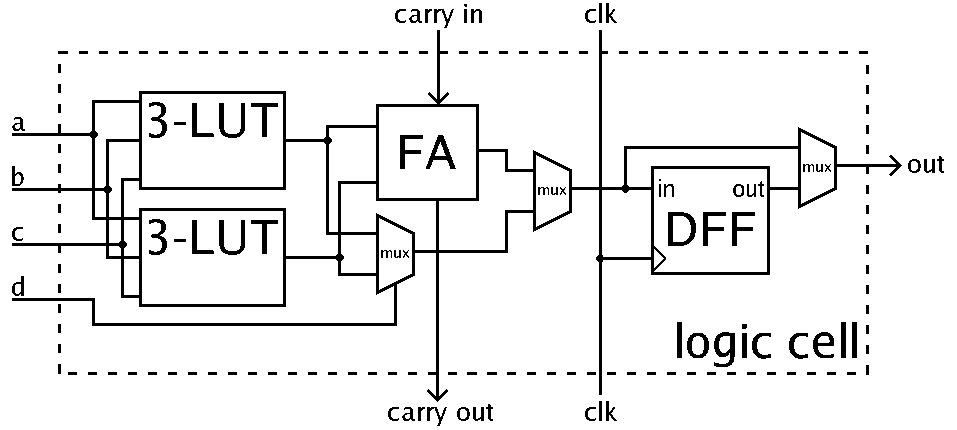
\includegraphics[width=1.0\linewidth]{images/chapter2/FPGA_cell_example.png}
\caption{Simplified schematic of a FPGA cell}
\label{fig:fpga_cell}
\end{figure}

A basic logic block consists of a few Logic Elements. As shown in figure \ref{fig:fpga_cell}, a Logic Elements is made of LUTs, a Full-Adder (FA), a D-Type Flip Flop and a bunch of multiplexers. This particular architecture can work in two modes: \textit{normal} mode and \textit{arithmetic} mode. Thanks to the Flip Flop, FPGAs can implement operations where some kind of memory is required.\bigskip

Modern FPGAs are very complex and expand upon the above capabilities to include other functionalities in silicon. Having these common functions embedded in the circuit reduces the area required and gives those functions increased speed compared to building them from logical primitives (because are implemented in-silicon, built out of transistor instead of LUTs, so they have ASICs-level performance). Examples of these include multipliers, generic DSP blocks, embedded processors, high speed I/O logic (like PCI/PCI-Express controllers, DRAM Controllers and so on and so forth) and embedded memories. \bigskip

Once the User's Application is designed (i.e. the description of the FPGA is written), the design needs to be mapped onto the FPGA's hardware resources. This is done using the Vendor's specific software and it's in charge of deciding which FPGA's LE is assigned to which subpart of the description and how each LE is configured. Then, all the LEs needs to be connected between themselfs and the I/O pads, and this is done by routing algorithms that decides the best way to connect them. Once all the implementation steps are done, a configuration file is generated that will eventually used to program the FPGA and is called \textit{bitstream}.\bigskip

All the programmable bits (like the content of the LUTs, some multiplexers selection signals or the routing details) are stored in the FPGA in memory elements that are outside the FPGA's funcional blocks (i.e. the one that can be used by the user to implement the application). Those memory elements can be though of as a big array of bits, or a \textit{shift register}. It's the \textit{configuration memory}: it stores the configuration bits of the entire FPGA and is loaded with the bitstream when the FPGA itself is programmed. Most FPGAs rely on an SRAM-based approach to be programmed: this allows to be in-system programmable (so the FPGA chip can be programmed without unmounting it from the board and from the system itself) and re-programmable (can be programmed as many times we want), but require external boot devices. Because the SRAM is a volatile memory, when the FPGA is powered off, the configuration memory content is lost. An external memory where the bitstream can be retrieved is required in order to re-program it. The SRAM approach is based on CMOS.\bigskip

Consequently, FPGAs are alternatives to hard-core CPUs. This means that on a FPGA a CPU can be implemented out of logic primitives (called \textit{soft-core}), alongside with the hardware that is used to implement the application like peripherals, memory and other components. Modern FPGAs supports \textit{at runtime programming}, this lead to the idea of \textit{reconfigurable systems}, where for example a CPU can be reconfigured in order to enable/disable some of its functionalities to suit the task at hand. The concept of \textit{reconfigurable systems} is also used in another manner and will be explained further in the next chapters.

\subsection{FPGAs vs. ASICs}

An \textit{ASIC} (application-specific integrated circuit) is an integrated circuit chip customized for a particular use. ASIC chips are typically fabricated using metal-oxide-semiconductor (MOS) technology. Thanks to the miniaturization of the MOS-based transistors and the improvement in the design tools, the maximum complexity (and hence functionality) possible in an ASIC has grown from 5000 logic gates to over 100 million. \bigskip

They are designed using the same HDLs Languages as the FPGAs, but the similarities stop there. Once the description is complete, specific ASIC softwares are used to synthesize and implement onto a technology library. While the corresponding technology library in FPGAs is simpler (made of LEs and routing elements), on ASICs it's a lot more complex. A typical ASIC technology library consists of a set of basic logic gates (like 2 input NAND, 3 input OR, 2 input FA, etc.) provided by the manufacturer that will manufactur the chip. Once a HDL description is mapped on top of the ASIC library, the so called \textit{gate-level netlist} is sent to the manufacturer. Here, ad-hoc technicians will start to work on this netlist, doing the \textit{route} {\&} \textit{place} of the netlist and as output of this process, a set of masks will be generated. The masks are used to \textit{print} the circuit in the silicon. On top of all this process, tests engineers must prepare a set of tests that in order to test the correct functionalities of the circuit during the various stages of the manufacturing process, until the end of the process itself. \bigskip

This allows to implement entire microprocessors, memories (including ROM, RAM, EEPROM and flash) and other large component in a single chip. Usually, for lower production volumes, FPGAs may be more cost-effective than an ASIC design. This is due to the non-recurring engineering (NRE) cost of an ASIC, that can run into millions of dollars. \bigskip

To recap:
\begin{itemize}
    \item ASICs circuits are faster, less power-hungry than FPGAs.
    \item ASICs are more complex to design and implement (hence more expensive) than FPGAs.
    \item FPGAs are more flexibile than ASICs.
\end{itemize}


\subsection{FPGA or ASIC in Aerospace Applications?}

In the aerospace industry, we are witnessing a turnaround in the last years regarding the hardware technology. FPGAs are typically much less radiation hardened than ASICs, so they are more prone to SEUs as well as lower total ionizing dose tolerance, but there are techniques to reduce these deficiencies. However, FPGAs are used on a lot more missions nowadays than 15 years ago, for all the reasons that make FPGAs a better choice than ASICs.\bigskip

As an example, Mars Exploration Rovers were something like 90\% ASICS. The last JPL's Martian Rover, Perserverance, is a very complex system and it's a very challenging design from the engineering point of view: it has multiple sensors and cameras to collect as much data as possible and, due to the volume of live data being recorded and the long data transmission time from Mars to Earth, a powerful processing system is essential. Early Mars rovers were basing their workload mainly on CPUs and ASICs as the processing units, while nowadays FPGAs are taking on much of the workload, like in Perseverance.\bigskip

There are different reasons behind this choice. The first one is the flexibility given by their re-programmability: because of the different stages a mission is made of, some parts of the system could be useful only in some of those stages (maybe intermediate ones) and they will never be used again. This is a waste of resources: FPGAs can be a great help in this aspect and Perserverance rover is an example. It utilizes an almost decade-old FPGA technology (Xilinx Virtex-5, introduced in May 2006 on 65 nm technology) as one of the main processing units. This unit is responsible for rover entry, descent and landing on Mars. Once the rover is landed, this unit would be useless and would become a \textit{dead hardware}. However, it's based on a FPGA hardware so it has been reprogrammed by NASA engineers from Earth to handle computer vision tasks.\bigskip

Other units on Perseverance such as radars, cameras, UHF transceivers, radar, and X-ray (used to identify chemicals) are controlled using Xilinx's FPGAs. Another interesting point is that Perserverance uses machine learning algorithm running on FPGAs, and they are so well optimized that it's achieving higher performance levels (about 18 times) than Curiosity rover (landed on Mars in 2012 and still active). \bigskip

Another advantage of using FPGAs is the faster time-to-space. There are different points that help in achieving this advantage. Not only the development on FPGA is faster than on ASICs (cost of design, development and fabrication of an ASIC are not present), but the most important thing is that there are many and many changes in the processing unit's architecture during project's development phase. There is usually a very stricted launch window for the mission that can be missed, and FPGAs help in two ways mainly:

\begin{itemize}
    \item Physically changing or adding more to a space system is a real challenge. The installation itself is not that difficult, but the system has to be recertified, proving that the it is still dependable. Furthermore, FPGAs simplify this greatly: the only thing to prove is that the FPGA chip is safe to fly with. Once this is done, the overall number of different parts to be certificied is reduced. Second, a change of the bitstream or of the software running on a \textit{soft-core} take a lot less time to certify.
    \item Software and Hardware development can be done in parallel. This is a great advantage for the software development team, because a first iteration of the hardware can be prepared and ready to use be used by the software team faster and the software team can start to work on the software itself.
\end{itemize}

FPGAs are not only helpful during the development phase, but even during the operational phase. Missions are prepared to last a relatively long time, but usually the quality of the work is so high that they last much longer. Examples are Mars rovers: Opportunity landed on the Red Planet in 2003 and it was ended by a martian dust storm in 2018, so it lasted for 15 years. Curiosity in 2012 and in 2022 is still active. This is a so long period that, speaking again about \textit{re-programmibility}, the processing system architecture may require changes to let the mission continue working. In fact, different things can go wrong in a decade and having a full reconfigurable system (from remote in particular) is a must, giving ground engineers a lot more possibilities to fix the system or to add/remove components. \bigskip

On the radiation tolerant side, vendors offer radiation-tolerant FPGAs. On top of that, it's possible to apply some logic changes to the design like TMR (Triple Module Redundacy) to a portion of the design or even to the entire design. Basically, it consists in triplicating the design and add a voter at the outputs. If a radiation error occurs, it will theoretically affect only one module so there will be two different results from the three modules (two correct and one wrong caused by the radiation). The voter will select the correct result (that is the majority). This is an example of making a design more robust to radiation.\bigskip

\section{Radiations}

We are going to understand better why radiation effects regarding electronic devices are one of the primary concerns for the aerospace industry.\bigskip

\subsection{Radiation sources}
Where does the radiation originate from? Unfortunately, the Universe and in particular the Solar System are full of radiations. The natural space radiation environment can damage electronic devices in different ways, ranging from a degradation in performances to a complete functional failure. More and more a space system goes deeper in the space, less and less it is protected by the Earth's atmosphere.\bigskip

Close to the Earth, there are two three sources of radiation: the Van Allen Belts, the Sun and the Cosmos itself. Van Allen Belts are zones of energetic charged particles, that are generated for example by the Sun, and captured by the Earth's magnetosphere. By trapping those charged particles, the magnetic field deflects them and protects the atmosphere from destruction. The two Earth's main belts extends from an altitude of 640 km to 58.000 km, in which radiation levels vary. Between the two belts, the \textit{inner} and the \textit{outer} there is a zone called \textit{safe zone} where the level of radiation is pretty low. Spacecrafts travelling beyond the LEO (Low Earth Orbit) go through the two belts, and beyond the belts they face additional hazards from cosmic rays and solar particle events (coronal mass ejections and solar flares).


\subsection{Radiation problems on Earth: the Nintendo's Super Mario 64 glitch}

Here on Earth, electronic devices are often not shielded or design to tolerate radiations. Usually, only safety-critical systems undergo the same kind of radiation-tolerant techniques as the ones used in the space system, like Aviation and Nuclear Power Plants, for instance.\bigskip

Even if there is a big magnetosphere protecting the planet's surface, some charged particles still escape and travel until they reach the ground and some everyday device. In 2013, a player was challenging another player in Nintendo's Super Mario 64 game. Suddenly, Mario was teleported into the air, saving crucial time and providing an incredible advantage in the game. The glitch caused the attention of a lot of players, and a \$1000 reweard was offered to anynone who could replicate the glitch. Users tried in vain to recreate the scenario, but no-one was able to emulate that giant leap. In the end, after eight years, user concluded that the glitch was not replicable because it was caused by a charged particle coming from the outer space that caused a bit-flip in the value that defines the player's height. \bigskip

Another curious case was the one related to the electronic voting machine in Belgium in 2003. A bit-flip here caused an adding of 4096 extra votes to a candidate. The error was only detected because there were more preferential votes than the candidate's own list, which is impossible in the voting system. The official explanation was ``the spontaneous creation of a bit at the position 13 in the memory of the computer''. It's not a coincidence that the value added was exactly 4096, in hexadecimal \texttt{0x1000}, that is $2^{12}$.

\subsection{Types of radiation}
The most common way to classify radiations is based on their effects on electronic devices. If the effect is the result of a cumulative damage (i.e. passage of many charged particles in different moments in time, and each particle has a relative low energy) then it can be a \textit{total ionizing dose} or a \textit{displacement ionizing dose}. If the effect is the result of a single charged particle (with a high energy) then it can be \textit{destructive} or \textit{non-destructive}, and they are usually referred as SEE (Single Event Effects). \bigskip

\subsubsection{Total ionizing dose}
Most electronic devices are based on MOS transistors, forming the basis for digital logic. The common way to use those transistors is as \textit{electronic switches}: there are two isolated contacts, the source and the drain (i.e. the switch is off, no current). When a positive charge is applied to the gate (in the case of a NMOS transistor), electrons (that are negative charges) are allowed to pass from the two isolated contacts (i.e. the switch is on). \bigskip

When ionizing radiations passes through the device, electrons are moved away from the material leaving 
``holes'' of missing charge, acting as positive charge carriers. These holes can find their way to the gate oxide and become trapped: this phenomenon is called \textit{total ionizing dose}. The effect of this phenomenon is the same as applying some positive voltage to the gate. With enough accumulated charges, the effect is to have the transistor always on, or better, in the \textit{stuck-on state}. \bigskip

\subsubsection{Displacement ionizing dose}
Another form of cumulative damage is the \textit{displacement ionizing dose}. This is the effect of a single charged particle passing through the device. What happens is that an atom is displaced from the material, modifying the crystal structure of the material itself. These microscopic effects create traps and recombination centers, eventually leading to the modification of the free flow of the current. This will ultimately impact the device's performance. \bigskip

\subsection{Single Event Effects}
When a single high-energy charged particle passes through the device, it can cause a \textit{destructive} or \textit{non-destructive} effect. The particle creates a momentary change of charge in the device, creating an unexpected current that can affect the device in various ways. Some effects may be completely destructive, while others may degrade performance to the point that the device doesn't work anymore in the limits required by the circuit or the system itself. Other effects cause the device to momentarily work in a wrong way, causing a functional failure (so it's not destructive from the point of view of the device but can cause an functional error, for example a wrong value in the memory from \textit{0xe} to \textit{0xf}). \bigskip

Within the destructive effect, the most common are Single Event Latchup (SEL), Single Event Burnout (SEB) and Single Event Gate Rupture (SEGR).

\subsubsection{Single Event Latchup}
In CMOS technology, there are a lot of intrinsic BJT (Bipolar Junction Transistor). When a special arrangement of PMOS and NMOS transistors is used, resulting in a n-p-n-p structures (corresponding to a NPN and a PNP transistor stucked next to each other), a CMOS Latchup structure is created. If one of these two transistor is activated (accidentally by a high-energy charged particle), the other one will be activated too, creating a feedback loop. They will both keep each other activated for a long as some current flows through them. This phenomenon will increase the current draw and can bring to the destrupution of the device. Usually, the only way to correct this situation is to make a \textit{power cycle}, so completely shutting down the device and then restarting it. However, latent damage may exists that may not appear until later. \bigskip

\begin{figure}[H]
\centering
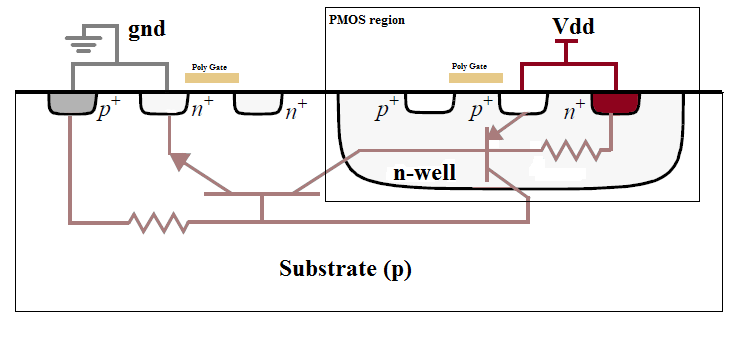
\includegraphics[width=1.0\linewidth]{images/chapter2/Latchup.png}
\caption{The intrisic BJTs in the CMOS Technology that can cause a Latchup. Deepon, CC BY-SA 3.0, via Wikimedia Commons}
\label{fig:latchup}
\end{figure}

\subsubsection{Single Event Burnout}
Can happen when an incident particle initiates an avalanche charge multiplication effect. This leads to an increasing current, leading to a thermal runaway of the device, causing local melting or ejection of molten material in a small-scale explosion. Obviously, the result is a complete destruction of the device. \bigskip

\subsubsection{Single Event Gate Rupture}
SEGR is the destructive rupture of a gate oxide (or any dielectric layer in a transistor). The effects can be observed in power MOSFETs with an increase of current flow when turned on, or in digital circuits with stuck bits. 

\subsubsection{Single Event Upset}
This is the most common non-destructive effect. As known as \textit{bit-flip}, it's caused by a particle that forces a digital signal to an opposite value momentarily. It can lean in a temporary modification of the digital output in a combinatory circuit, and the modified value can be memorized in a flip-flop or any other memory element if sampled at the same time a radiation arrives. In more complex circuits, it can cause other malfunctions like resets and memory values modifications. \bigskip

\begin{figure}[H]
\centering
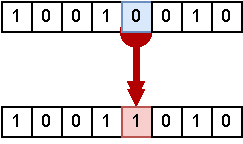
\includegraphics[height=0.2\linewidth]{images/chapter2/SEU_EXAMPLE.pdf}
\caption{Example of a Single Event Upset in a memory element.}
\label{fig:seu_example}
\end{figure}

What is shown in Figure \ref{fig:seu_example} can for example happen in a SRAM memory. Each cell is made of a cross-coupled transistors. Each side couple are connected forming an inverter (NOT logic function), and the output of the inverter is connected to the gates of the second couple.  

\begin{figure}[H]
\centering
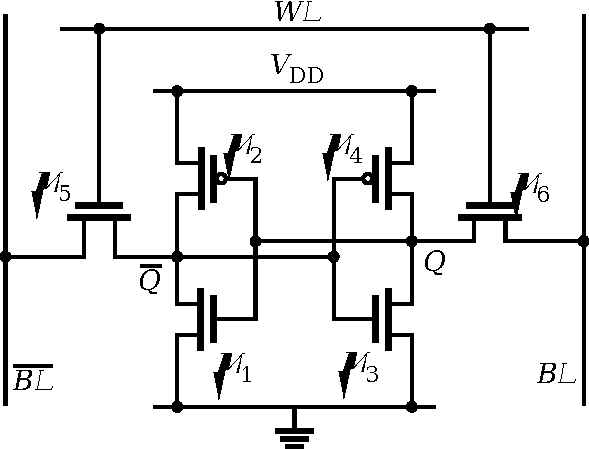
\includegraphics[height=0.4\linewidth]{images/chapter2/SRAM_CELL.pdf}
\caption{Simple SRAM Cell layout. Inductiveload, Public domain, via Wikimedia Commons.}
\label{fig:sram_cell_layout}
\end{figure}

In Figure \ref{fig:sram_cell_layout}, a simple layout is proposed. In order to have a logic 0 as output (\textit{BL = 0}), M3 is active (thus M4 is not active). So M2 is active (thus M3 is not active). If a radiation strikes one of those transistor, can happen that the M3's gate voltage goes low, causing a flip of the configuration thus a flip of the stored bit. \bigskip

As explained in Section \ref{sec:fpgaarchitecture}, most FPGAs' memory configuration are based on SRAM technology. If a bitflip occurs, the FPGA configuration itself is modified, leading to a malfunction of a module or to a routing modification.\bigskip

% Explain why the trends (smaller transistors) cause SEU to be more common than accumulation effects.
\chapter{Hello}
\label{sec:hello}

% use [][] to prepend/postpone text to the citation
\cite[Hi][Goofy]{IEEEexample:article_typical}

\si{\kilo\gram\per\second}

% generic figure
\begin{figure}[h]
\centering

\includegraphics[width=.9\linewidth]{images/logo/logoPoliTo_with_name_wrong.png}
\caption{Hi}
\label{fig:hi}
\end{figure}

% use [] to set name for ToC
\section[Extremely long name with manual linebreak which otherwise would not fit the page]{Extremely long name with manual linebreak\\which otherwise would not fit the page} % ok with fontsize=12pt

% list
\begin{enumerate}
    \item A
    \item B
    \item C
\end{enumerate}

% minipage to put two images in the same figure
\begin{figure}[h]
    \centering
    \begin{minipage}[t]{.49\linewidth}
    \begin{figure}[H]
	\centering
	
\includegraphics[width=\linewidth]{images/logo/logoPoliTo_with_name_low_quality.jpg}
	\caption{HI}
	\label{fig:c}
    \end{figure}
    \end{minipage}
    \hfill
    \begin{minipage}[t]{.49\linewidth}
    \begin{figure}[H]
	\centering
	% svg inclusion, requires inkscape
	\includesvg[width=\linewidth]{images/artificial_neural_network.svg}
	\caption{SVG}
	\label{fig:svg}
    \end{figure}
    \end{minipage}
\end{figure}

\begin{table}[]
    \centering
    \setcellgapes{3pt}
    \makegapedcells
    \begin{tabular}{|c|c|c}
    \hline
    ReLU & $f(x) = \begin{cases}
	0 & \text{for } x \le 0\\
	x & \text{for } x > 0\end{cases}$ \\ \hline
    Softmax & $f_i(\vec{x}) = \dfrac{e^{x_i}}{\sum_{j=1}^J e^{x_j}} i = 1, ..., J$ \\ \hline
    tanh & $f(x)=\tanh(x)=\dfrac{(e^{x} - e^{-x})}{(e^{x} + e^{-x})}$ \\ \hline
    \end{tabular}
    \caption{Examples of activation functions, operating either element-wise or vector-wise, depending on the function}
    \label{tab:activation_functions}
\end{table}

\begin{equation}
    \label{eq:fully_connected}
    output = f_{activation}\left(\displaystyle\sum_{\#neurons} input_i + bias\right)
\end{equation}

\begin{table}
    \centering
    \begin{adjustbox}{width={0.9\textwidth},totalheight={\textheight},keepaspectratio} % needed if the table overflows the margins, requires adjustbox package
    \setcellgapes{3pt}
    \makegapedcells
    \begin{tabular}{|c|c|}
    \hline
    MSE / L2 Loss / Quadratic Loss & $\dfrac{\sum_{i=1}^{N} \left(y_i - \hat{y}_i\right)^2}{N}$ \\ \hline
    \makecell{(Binary) Cross Entropy \\ (average reduction on higher dimensions)} & $\dfrac{\sum_{i=1}^{N} \sum_{j=1}^{C} \hat{y}_i \log\left(y_{i,j}\right)}{N}$ \\ \hline
    \makecell{Categorical Cross Entropy \\ (sum reduction on higher dimensions)} & $- \sum_{i=1}^{N} \hat{y}_i +  \log\left(\sum_{i=1}^{N} \sum_{j=1}^{C} y_{i,j}\right)$ \\ \hline
    \end{tabular}
    \end{adjustbox} % must be closed before label and caption
    \caption{$y$ is the output of the network, $N$ is the batch size multiplied by the number of outputs (e.g. pixels), $C$ is the number of classes and $\hat{y}$ is the correct output.}
    \label{tab:loss_functions}
\end{table}


\begin{algorithm}
\caption{Adam optimizer algorithm. All operations are element-wise, even powers. Good values for the constants are $\alpha=0.001, \beta_1 = 0.9, \beta_2 = 0.999, \epsilon = 10^{-8}$. $\epsilon$ is needed to guarantee numerical stability.}
\label{alg:adam_optimizer}
\begin{algorithmic}[1]
\Procedure{Adam}{$\alpha, \beta_1, \beta_2, f, \theta_0$}
\LineComment{$\alpha$ is the stepsize}
\LineComment{$\beta_1, \beta_2 \in \left[0, 1\right)$ are the exponential decay rates for the moment estimates}
\LineComment{$f\left(\theta\right)$ is the objective function to optimize}
\LineComment{$\theta_0$ is the initial vector of parameters which will be optimized}
\LineComment{Initialization}
\State $m_0 \gets 0$
\Comment{First moment estimate vector set to 0}
\State $v_0 \gets 0$
\Comment{Second moment estimate vector set to 0}
\State $t \gets 0$
\Comment{Timestep set to 0}
\LineComment{Execution}
\While{$\theta_t$ not converged}
\State $t \gets t + 1$
\Comment{Update timestep}
\LineComment{Gradients are computed w.r.t the parameters to optimize}
\LineComment{using the value of the objective function}
\LineComment{at the previous timestep}
\State $g_t \gets \nabla_\theta f\left(\theta_{t - 1}\right)$
\LineComment{Update of first-moment and second-moment estimates using}
\LineComment{previous value and new gradients, biased}
\State $m_t \gets \beta_1 \cdot m_{t - 1} + \left( 1 - \beta_1 \right) \cdot g_t$
\State $v_t \gets \beta_2 \cdot v_{t - 1} + \left(1 - \beta_2 \right) \cdot g_t^2$
\LineComment{Bias-correction of estimates}
\State $\hat{m}_t \gets \dfrac{m_t}{1 - \beta_1^t}$
\State $\hat{v}_t \gets \dfrac{v_t}{1 - \beta_2^t}$
\State $\theta_t \gets \theta_{t - 1} - \alpha \cdot \dfrac{\hat{m}_t}{\sqrt{\hat{v}_t} + \epsilon}$
\Comment{Update parameters}
\EndWhile
\State \textbf{return} $\theta_t$
\Comment{Optimized parameters are returned}
\EndProcedure
%\end{small}
\end{algorithmic}
\end{algorithm}

% bullet points
\begin{itemize}
    \item A
    \item B
    \item C
\end{itemize}



% \paginavuota % it works even without stile=classica

\appendix
% appendix
\chapter{Galileo}
\label{sec:appendix_galileo}

%\lstinputlisting[]{} % for source code files directly
% lstlisting environment for direct inclusion
\begin{lstlisting}[language=Python]
    import os
    os.system("echo 1")
\end{lstlisting}

% for computational complexity
$\mathcal{O}\left(n\log{n}\right)$

% verbatim
\verb+numpy+



% endnotes here if needed

\phantom{0}
\cleardoublepage
\printbibliography[heading=bibintoc] % heading required to show it in ToC

\end{document}
